\documentclass[conference]{IEEEtran}
\IEEEoverridecommandlockouts
\usepackage[table]{xcolor}
\usepackage{cite}
\usepackage{amsmath,amssymb,amsfonts}
\usepackage{algorithmic}
\usepackage{graphicx}
\usepackage{textcomp}
\usepackage{booktabs}
\usepackage{multirow}
\usepackage{array}
\graphicspath{{./}}
\def\BibTeX{{\rm B\kern-.05em{\sc i\kern-.025em b}\kern-.08em
    T\kern-.1667em\lower.7ex\hbox{E}\kern-.125emX}}

\begin{document}

\title{SSM-Psychiatrist: A Slot State Machine-Governed Agent for Clinical Psychiatric Interviews%
\thanks{This work was supported by the Beijing Jiaotong University Natural Science Talent Fund Project (Grant No.~2025JBRC014).}}

\author{
\IEEEauthorblockN{Anonymous Author(s)}
\IEEEauthorblockA{
\textit{Institution anonymized for review}\\
anonymized@review.org}
}

\maketitle

% ============================================================
\begin{abstract}
% ============================================================
Structured psychiatric intake interviews impose a completeness
requirement that large language models (LLMs) cannot satisfy by design:
all diagnostically critical information must be collected and verified
before a clinical record is generated. Prompt engineering and model
scaling do not resolve this deficiency, because LLMs possess no
internal coverage criterion and terminate interviews stochastically. We
present \textbf{SSM-Psychiatrist}, a dual-component agent that enforces
procedural coverage with respect to an explicit slot taxonomy. A Slot State Machine (SSM)
component maintains a four-state coverage model over each clinical slot
(Empty, Filled, Refused, or Unknown) across a DSM-5-TR-grounded slot
taxonomy of 120 clinical slots spanning eleven diagnostic categories,
applies three evidence-triggered priority rules for risk
stratification, diagnostic criterion gating, and differential diagnosis
escalation, and gates medical record generation behind a three-condition termination criterion. An LLM execution
component operates solely as a surface generator under SSM directives,
with no authority over coverage decisions. We evaluate SSM-Psychiatrist
on the Psychiatric Interview Benchmark (PIB), a 110-case multi-turn
clinical interview suite we construct that covers eleven DSM-5-TR
diagnostic categories. SSM-Psychiatrist achieves \textbf{97.3\% dynamic
Top-1 diagnostic accuracy} with 100\% must-ask slot coverage and 100\%
SVCL domain coverage under the PIB protocol, whereas all nine evaluated
frontier LLM baselines receive a dynamic Top-1 score of 0.000 under the
same protocol despite reaching up to 95.5\% static diagnostic accuracy.
The reported dynamic Top-1 metric is end-to-end: it includes
structured-output compliance and should not be interpreted as diagnostic
correctness alone. The results motivate the proposed enforcement
mechanisms, while clinical validity, semantic extraction accuracy, and
generalization beyond synthetic cases require separate evaluation.
\end{abstract} 

\begin{IEEEkeywords}
clinical interview system, slot state machine, coverage guarantee, procedural coverage, LLM failure modes, DSM-5-TR, medical AI, dialogue state tracking.
\end{IEEEkeywords}


% ============================================================
\section{Introduction}
% ============================================================
Large language models (LLMs) can now sustain multi-turn clinical dialogue~\cite{tu2025towards,johri2025evaluation}, encode substantial medical knowledge~\cite{thirunavukarasu2023large}, and execute extended clinical tasks as autonomous agents~\cite{kim2024mdagents,ferber2025development}. Psychiatric care is a natural fit: unlike many specialties, the core of a psychiatric assessment is the patient's own account, gathered through \emph{structured interviews}~\cite{abi2023candidate,hua2025charting}. The standard diagnostic workflow is shown in Fig.~\ref{fig:clinical_workflow}.

\begin{figure}[t]
\centerline{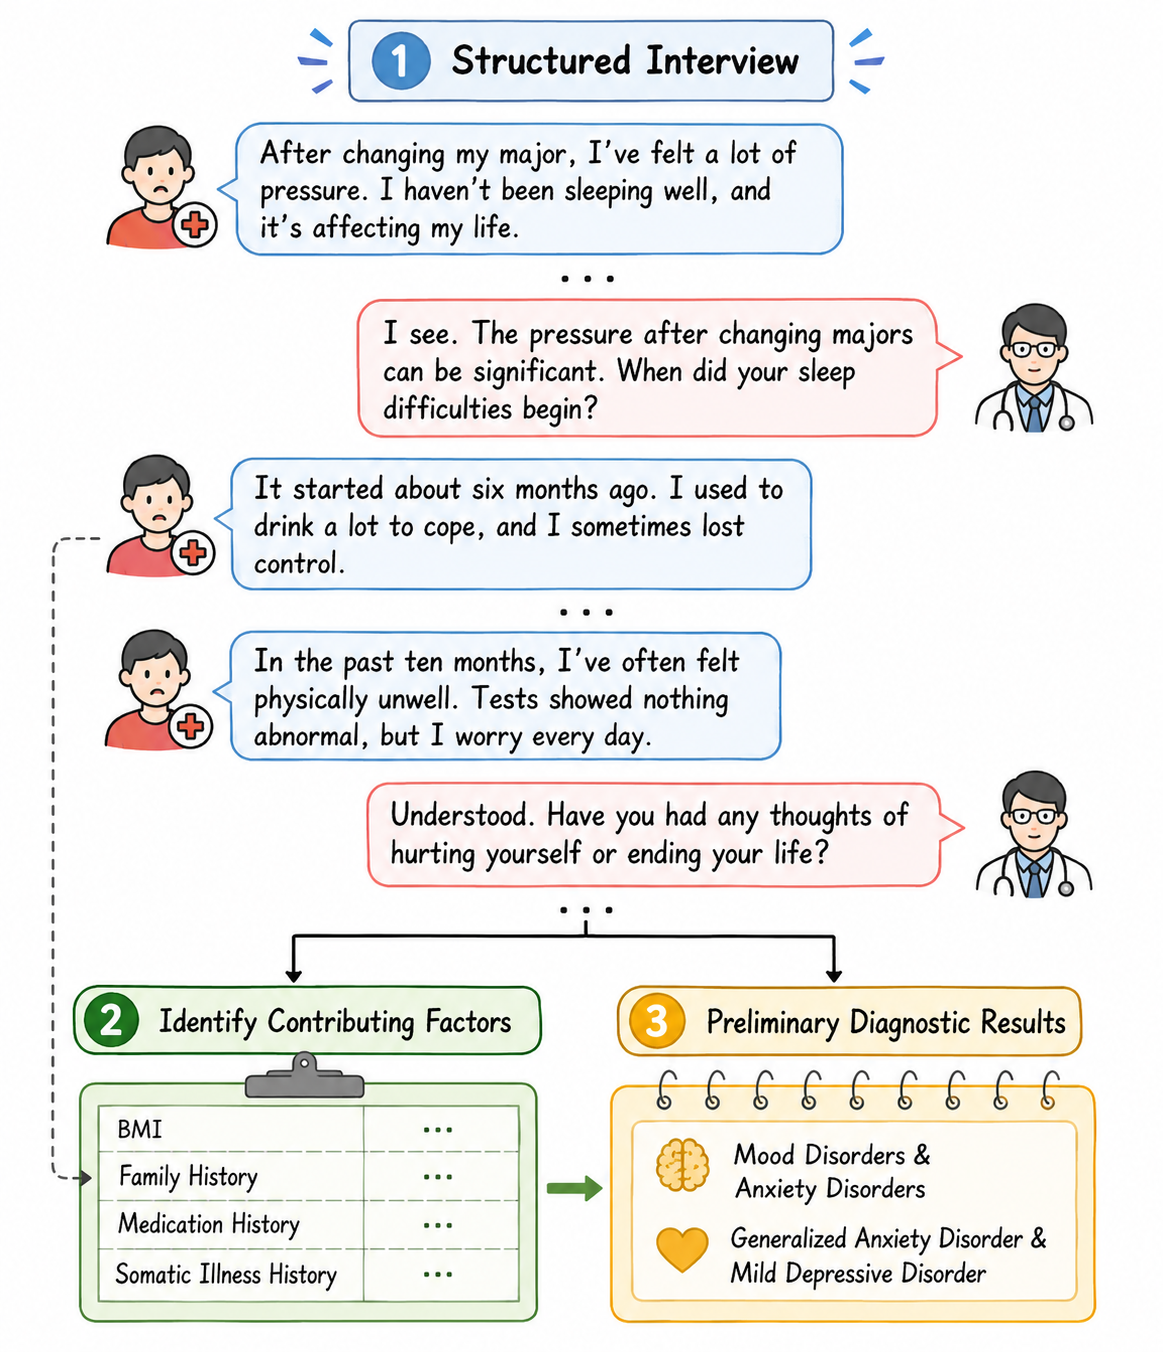
\includegraphics[width=\columnwidth]{a82f1f3d-28d8-454a-8a91-a8302fc96702.png}}
\caption{Standard psychiatric diagnostic workflow.
\textbf{(1) Structured Interview}: multi-turn dialogue collecting patient-reported symptoms and psychosocial context.
\textbf{(2) Contributing Factors}: objective clinical data (BMI, family history, medication history) activate evidence-triggered priority rules.
\textbf{(3) Diagnostic Results}: structured medical record with differential diagnoses upon interview completion.}
\label{fig:clinical_workflow}
\end{figure}

However, deploying an LLM as the interviewer surfaces a requirement that conversational fluency does not address. When a clinician conducts a structured intake interview, two guarantees are implicit: every required question is asked with omissions recorded, and the interview does not end until a threshold of diagnostic completeness is reached. Safety-critical items such as suicidal ideation are always raised regardless of conversational flow, and the decision to stop is a clinical judgment grounded in validated instruments (e.g., SCID-5-CV~\cite{first2015structured}, MINI~\cite{sheehan1998mini}).

Current LLM-based interviewers possess neither guarantee. First, an LLM
cannot articulate why it stopped: it has no completeness
criterion, only a next-token distribution, so termination is a
byproduct of generation rather than a verified state. Second, it cannot
ensure that every required item has been addressed to a clinical
standard, because nothing constrains the conversation to cover the
mandated questions. The consequences are concrete: an LLM may produce a
plausible medical record after four turns without ever asking about
suicidal ideation, or judge a depressive presentation primary without
screening for the obsessive-compulsive ideation that better explains
it.  We term this the \emph{clinical coverage guarantee problem}: the
inability of a language model, operating alone, to certify that an
interview has reached a sufficient state. This is a matter of
architecture rather than model capability alone, since a more capable
model still lacks an externally verified coverage criterion and a
richer prompt remains probabilistic. The proposed solution is therefore
structural, but its clinical adequacy remains conditional on the
taxonomy, extraction quality, and governance rules.

Two categories of engineering responses to these problems exist in practice, and both are inadequate. \textit{Rigid scripted systems} (electronic PHQ-9, GAD-7 questionnaires) solve coverage by enumeration: present every question in a fixed order. The guarantee is real, but the cost is that the system cannot adapt to patient responses---it cannot escalate on a safety signal, reorder questions based on emerging clinical evidence, or adjust its communication style for patient affect. The result is low adherence, particularly in psychiatric populations~\cite{torous2020dropout}.

\textit{Prompt-engineered LLM systems} attempt to solve coverage by instruction: tell the model to ask all required questions. This fails for three reasons. First, instructions compete with conversational coherence. Second, LLM compliance with coverage instructions is not verifiable at runtime. Third, LLMs systematically omit certain content categories---residual diagnostic labels, explicit safety probes---from their responses under naturalistic conversational pressure~\cite{ni2026disentangling}, a pattern we reproduce empirically in Section~\ref{sec:failuremodes}.

We address this with \textbf{SSM-Psychiatrist}, an agent built on a strict architectural division: coverage governance and conversational generation are handled by separate components that share no responsibilities:
\begin{enumerate}
  \item \textbf{The Slot State Machine (SSM) component} is the coverage
  authority. It tracks the formal completion state of all clinical
  slots, applies evidence-triggered priority rules that reorder the
  collection agenda in response to patient disclosures, and enforces a
  three-condition termination criterion that the LLM cannot override.
  \item \textbf{The LLM execution component} is the surface generator.
  Given a collection directive from the SSM, it produces contextually
  appropriate natural language (empathic, adaptive, grammatically
  coherent) with no responsibility for coverage decisions.
\end{enumerate}
The agent is grounded in a DSM-5-TR-aligned slot taxonomy for
multi-domain psychiatric assessment. We evaluate it on the Psychiatric
Interview Benchmark (PIB), a multi-turn clinical interview benchmark we
construct for this purpose (Section~\ref{sec:dataset}), The evaluation
examines four LLM clinical-interview failure modes under a synthetic,
protocol-specific setting; it is not evidence of autonomous clinical
deployability or of state-of-the-art performance on a common benchmark.

% ============================================================
\section{Related Work}
% ============================================================

\subsection{LLM Agent Architectures}

Several LLM agent paradigms have been adapted for clinical use, each with a characteristic blind spot. ReAct~\cite{yao2022react} interleaves reasoning with environment actions to enable multi-step execution, but termination and topic coverage remain entirely at the LLM's discretion. LLM-assisted knowledge graph construction~\cite{yang2024kgllm} can encode clinical domain knowledge into structured workflows, yet the LLM still decides which graph nodes to traverse and when traversal is complete---slot coverage is never formally verified. Retrieval-augmented generation grounds responses in retrieved evidence~\cite{zhan2024rarok} but cannot compel the model to elicit specific information from a patient. Multi-agent pipelines~\cite{kim2024mdagents,liu2024medgen} distribute reasoning across specialized agents, improving answer quality; no agent in any such pipeline holds authority to certify that a session has reached clinical completeness or to block an early exit. In each case, the coverage decision is a probabilistic LLM output. That is precisely what makes the clinical coverage guarantee problem unsolvable within these paradigms alone.

\subsection{Safety and Completeness in Conversational AI}

Existing safety work for LLM-based systems addresses individual model outputs: safety alignment training~\cite{ouyang2022training}, content filtering~\cite{gehman2020realtoxicity}, and malevolent response detection in mental health dialogues~\cite{xu2024malevolence}. These output-level approaches are insufficient for clinical interviews, where safety is a session-level property: safety-critical items---such as suicidal ideation probes---must be asked and recorded across a multi-turn conversation regardless of how the dialogue unfolds. No output-level filter can enforce this, because the failure mode is omission rather than harmful output. Our SSM addresses this through mandatory safety gating: safety-critical slots are assigned the highest scheduling priority and cannot be bypassed by the LLM execution layer.

\subsection{Structured Clinical Interviews and Automation Approaches}

Structured psychiatric interviews---such as SCID-5-CV~\cite{first2015structured} and MINI~\cite{sheehan1998mini}---provide coverage guarantees through exhaustive enumeration: every required item is administered in a fixed order. This guarantee is real but brittle: rigid scripted systems cannot adapt to patient responses, escalate on safety signals, or reorder questions based on emerging clinical evidence, resulting in low adherence in psychiatric populations~\cite{torous2020dropout}. Attempts to automate structured interviews with prompt-engineered LLMs address the adaptability problem but sacrifice the coverage guarantee: LLM compliance with coverage instructions is not verifiable at runtime, and models exhibit systematic avoidance of certain question categories under naturalistic conversational pressure. Our SSM recovers the coverage guarantee of structured instruments while preserving the conversational flexibility of LLM-based systems, by separating coverage governance from language generation into two components with strictly partitioned responsibilities.

\subsection{Medical LLM Benchmarks and Their Limitations}

Existing medical LLM benchmarks---MedQA~\cite{jin2021disease}, PubMedQA~\cite{jin2019pubmedqa}, MedMCQA~\cite{pal2022medmcqa}, MultiMedBench~\cite{singhal2023large}---and psychiatric-specific systems~\cite{ding2025dale,li2025prenatal,xing2024emo,wang2024scalecot} uniformly evaluate \textit{diagnostic reasoning over pre-collected information}, conflating two distinct capabilities: diagnostic knowledge and information acquisition. Benchmarks testing only the former reveal little about clinical deployability. The PIB benchmark (Section~\ref{sec:dataset}) addresses this gap with dynamic multi-turn evaluation requiring models to conduct interviews from a minimal chief complaint. PIB comprises 110 synthetic cases across 11 DSM-5-TR diagnostic categories (10 per label), each constructed to satisfy the target diagnostic criteria while embedding realistic comorbidity signals and confounding symptom constellations that challenge differential diagnosis. A simulated patient agent responds according to per-case scripts, and each case is annotated with 120 clinical slots organized along the SVCL evaluation framework. To prevent oracle leakage, no baseline receives access to ground-truth labels, slot values, or rubric contents at runtime. A text contamination audit confirmed zero overlap with known public corpora.


% ============================================================
\section{The Clinical Coverage Guarantee Problem: A Formal View}
% ============================================================

\subsection{Interview as a Coverage Problem}

Let $\mathcal{S} = \{s_1, \ldots, s_N\}$ be the set of clinical slots required for a complete interview, each carrying a data type $\tau_i \in \{\text{Boolean}, \text{ordinal}, \text{categorical}, \text{duration}\}$. Define the \textit{coverage state} as:
\[
\Sigma^{(t)} = \bigl(\sigma_1^{(t)}, \ldots, \sigma_N^{(t)}\bigr),\quad \sigma_i^{(t)} \in \{\texttt{E}, \texttt{F}, \texttt{R}, \texttt{U}\}
\]
where \texttt{E} = empty (not yet addressed), \texttt{F} = filled (value obtained), \texttt{R} = refused (patient declined), \texttt{U} = unknown (patient unable to answer). An interview achieves \textit{full coverage} when $\forall i: \sigma_i^{(t)} \neq \texttt{E}$.

The coverage guarantee problem is: given that the LLM action at turn $t$ is drawn from a distribution conditioned on the conversation history, no finite prompt can guarantee $\Pr[\forall i: \sigma_i^{(T)} \neq \texttt{E}] = 1$ for any stochastic termination time $T$. A deterministic coverage authority is required. Such an authority can guarantee state completion relative to $\mathcal{S}$, but it cannot by itself guarantee that $\mathcal{S}$ is clinically exhaustive or that a non-empty state contains a semantically correct value.

\subsection{Coverage Failure Modes}

We identify four coverage failure modes that a clinical interview system must prevent:

\textbf{CF-1 (Premature Termination):} The system concludes the interview before all slots reach non-empty states.

\textbf{CF-2 (Safety Slot Omission):} Safety-critical slots (suicidal ideation, self-harm, violence risk) are not reached because the conversational flow prioritizes other topics first.

\textbf{CF-3 (Differential Diagnosis Blindness):} The system fails to escalate to differential diagnosis slots when symptom presentations are ambiguous, defaulting to the most salient diagnostic hypothesis.

\textbf{CF-4 (Output Verification Failure):} The system generates a final diagnostic output that fails structural validation, triggering fallback to a non-informative default.

Each failure mode appears empirically in PIB evaluation data, as we document in Section~\ref{sec:failuremodes}. Each corresponds to a specific mechanism in our SSM design.

\subsection{Termination Criterion Design}

For this system, record generation is authorized only when three conjunctive procedural conditions are satisfied:
{\small\[
\Phi(\Sigma) \triangleq \underbrace{\forall i:\ \sigma_i \neq \texttt{E}}_{\text{(C1) coverage}} \;\wedge\; \underbrace{\mathsf{SafetyComplete}(\Sigma)}_{\text{(C2) safety}} \;\wedge\; \underbrace{\mathsf{PathComplete}(\Sigma)}_{\text{(C3) Dx path}}
\]}
The SSM evaluates $\Phi$ after every turn. If $\Phi(\Sigma^{(t)}) = \texttt{False}$, record generation is blocked and the SSM issues a collection directive for the highest-priority remaining slot. The LLM has no mechanism to assert $\Phi$ independently; the termination authority resides entirely in the SSM. This is a guarantee of state-transition coverage relative to the predefined taxonomy, not a guarantee of clinical correctness, diagnostic validity, or safe autonomous care.


% ============================================================
\section{System Architecture}
% ============================================================

\subsection{Architectural Principle: Authority Separation}

The central design principle is \textit{authority separation}: coverage decisions and language generation are made by different subsystems communicating through a narrow interface (the collection directive). This differs from prompt-based approaches in which a single model simultaneously manages coverage tracking, priority scheduling, safety assessment, and natural language generation---tasks that create competing objectives within a single inference pass.

The system comprises four layers illustrated in Fig.~\ref{fig:architecture}. The \textit{user interaction layer} presents a natural language interface. The \textit{LLM execution layer} receives a collection directive from the SSM, produces a patient-facing utterance, and extracts slot values from patient responses. The \textit{SSM layer} applies state transitions, trigger rules, and the termination criterion. The \textit{data persistence layer} maintains immutable logs of all slot state transitions with supporting utterances for clinical audit.

The interface between layers is strictly unidirectional in terms of authority: the LLM cannot modify SSM state directly, and the SSM cannot generate language. The SSM can therefore preserve its procedural gating logic across execution models; nevertheless, question quality and semantic extraction remain model-dependent and must be monitored.

\begin{figure*}[!t]
\centerline{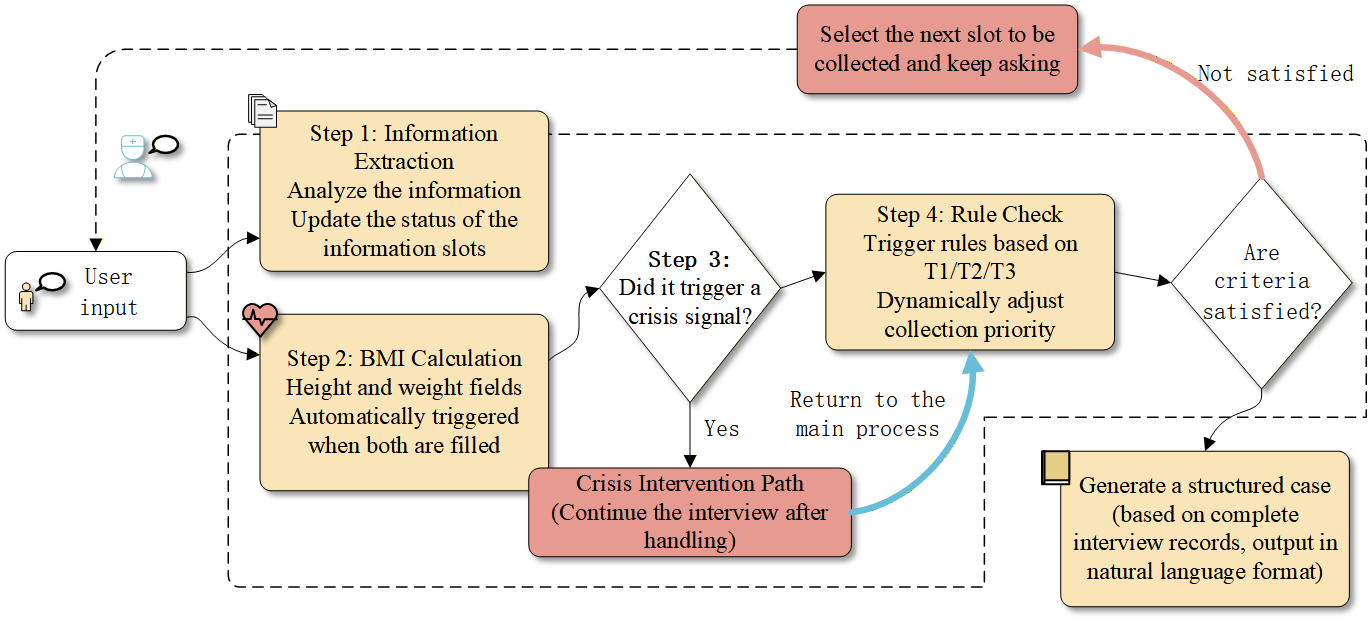
\includegraphics[width=\textwidth]{architecture.png}}
\caption{End-to-end flow of the SSM-guided psychiatric interview agent.
The SSM layer holds exclusive authority over slot state transitions,
trigger rule evaluation, and the $\Phi$ termination criterion.
The LLM execution layer acts solely as a surface generator.
The data persistence layer maintains an immutable per-slot evidence log.}
\label{fig:architecture}
\end{figure*}

\subsection{Four-State Slot Model and Its Clinical Rationale}

Standard DST systems represent slots as either filled or empty. We introduce two additional states. \texttt{Refused} captures the case where the patient explicitly declines to answer---a clinically significant disclosure that should be recorded, not silently dropped. \texttt{Unknown} captures the case where the patient genuinely lacks the information. Both states are \textit{valid terminal states}: they advance the coverage count toward $\Phi$ without requiring a factual answer, preventing infinite re-querying that would block interview termination. They do not, however, resolve clinical uncertainty: for safety-critical slots, a refusal or unknown response must be retained in the record and trigger a predefined escalation or human-review pathway rather than be interpreted as a negative risk finding.

\subsection{Evidence-Triggered Priority Rules}

Normal slot scheduling follows a clinical priority ordering (safety slots first, then demographics, then primary complaint, then differential). Three hard-wired rules interrupt this ordering when specific clinical signals are detected.

\textbf{T1} responds to risk stratification indicators (e.g., elevated BMI, sleep apnea cues) by elevating relevant objective history slots to the top of the collection agenda.

\textbf{T2} implements a gating structure over the primary DSM-5-TR diagnostic criteria for the target condition, verifying each necessary criterion before the interview advances past the primary complaint module.

\textbf{T3} responds to semantic patterns associated with comorbid psychiatric presentations and temporally proximate stressor disclosures, mandating differential diagnosis slot collection before the interview can conclude---preventing CF-3.

The three rules may all fire within the same interview, producing a dynamically reordered collection agenda that reflects accumulated clinical evidence---a form of lightweight online clinical reasoning independent of LLM judgment.

\subsection{Non-Informative Response Handling}

A patient giving a non-informative response leaves the current slot in the \texttt{empty} state, blocking coverage progress. The LLM execution layer applies a progressive recovery sequence: (1) concrete numerical reframing, (2) social normalization, (3) behavioral rather than subjective framing, (4) third-party perspective elicitation, and (5) graceful slot closure at \texttt{unknown} after a bounded number of attempts. The bounded retry limit ensures deterministic termination, preventing CF-1 in the degenerate case of a consistently non-responsive patient.

\subsection{Dual-Phase LLM Invocation}

Cloud-based LLM providers apply content safety classifiers that may suppress responses containing descriptions of self-harm or suicidal ideation---necessary for consumer applications but obstacles in clinical contexts. We address this with a dual-phase invocation strategy: patient language is transmitted verbatim during the interview phase; a clinical terminology substitution pass is applied only during the record generation phase before API transmission. The verbatim patient language is preserved in the local evidence store. This enables safe elicitation without triggering content safety interventions, but it does not replace provider safeguards, local safety protocols, or clinician supervision.

\subsection{DSM-5-TR Knowledge Injection via Slot Taxonomy}
\label{sec:dsm_injection}

SSM-Psychiatrist instantiates the generic SSM framework with a DSM-5-TR-grounded slot taxonomy comprising 120 clinical slots organized across eleven diagnostic categories (Adjustment Disorder, BDD, BPD, IED, OCD, OCPD, OS-OCRD, PGD, PMDD, SSD, and Other) and nine SVCL domains. DSM-5-TR diagnostic criteria are encoded at two levels.

At the \textit{slot level}, each slot is derived from a specific DSM-5-TR criterion or specifier. For example, the criterion set for OCD (DSM-5-TR F42.2) maps to slots covering \texttt{obsession\_content}, \texttt{compulsion\_type}, \texttt{time\_consumed\_per\_day}, \texttt{distress\_level}, and \texttt{ego\_dystonia}. For BPD (F60.3), nine criterion-derived slots cover identity instability, interpersonal dysregulation, affective instability, impulsivity, and self-harm history. The MUST\_SLOTS designation for each diagnostic group is determined directly by the A-criteria listed in DSM-5-TR; specifiers and associated features map to group-specific slots.

At the \textit{trigger rule level}, DSM-5-TR diagnostic hierarchy and exclusion rules are encoded in T2 and T3. T2 implements the ``better explained by'' exclusion logic: when primary criterion slots for a candidate diagnosis are filled, T2 mandates collection of exclusion criterion slots before advancing. T3 implements the differential diagnosis gating from DSM-5-TR comorbidity guidelines, activating condition-specific slot groups upon detection of semantic patterns indicating comorbid presentations.

This design was first validated in a deployed clinical sleep medicine interview system using a 58-slot taxonomy (Insomnia Disorder F51.01, OSA G47.33, RLS G25.81, Parasomnias) with the same MUST\_SLOTS / group-specific layered design and T1--T3 gating. Extension to multi-domain psychiatric assessment required only slot taxonomy expansion, confirming the domain-agnostic nature of the SSM framework.Whether this transfer preserves clinical completeness or usability remains an empirical question.



% ============================================================
\section{LLM Failure Modes and SSM Design Justification}
\label{sec:failuremodes}
% ============================================================

\subsection{Evaluation Dataset}
\label{sec:dataset}

We evaluate SSM-Psychiatrist on the Psychiatric Interview Benchmark (PIB), a multi-turn clinical interview evaluation suite designed to assess both diagnostic knowledge and information acquisition capability in LLM-based interview agents. As the benchmark is not yet publicly released, we describe its design in full here.

\subsubsection{Case Construction}

PIB comprises 110 synthetic psychiatric cases spanning eleven diagnostic categories: Adjustment Disorder, Body Dysmorphic Disorder (BDD), Borderline Personality Disorder (BPD), Intermittent Explosive Disorder (IED), Obsessive-Compulsive Disorder (OCD), Obsessive-Compulsive Personality Disorder (OCPD), Other Specified OCD-Related Disorder (OS-OCRD), Prolonged Grief Disorder (PGD), Premenstrual Dysphoric Disorder (PMDD), Somatic Symptom Disorder (SSD), and an Other category covering atypical or mixed presentations. Each case is constructed to satisfy DSM-5-TR diagnostic criteria for the target category while embedding realistic comorbidity signals and confounding symptom constellations that challenge differential diagnosis. Diagnostic labels follow a controlled vocabulary aligned to DSM-5-TR ICD-10-CM codes.

The category selection targets the high-confusability region of DSM-5-TR nosology~\cite{apa2022dsm5tr}. Four categories occupy the OCD and Related Disorders chapter (OCD, OCPD, BDD, OS-OCRD), a grouping whose defining criterion---obsessional cognitions paired with repetitive behaviors or avoidance---creates a dense symptom-overlap space requiring systematic pairwise discrimination that existing medical LLM benchmarks do not assess~\cite{jin2021disease,jin2019pubmedqa,pal2022medmcqa}. The remaining seven categories span five additional DSM-5-TR chapters (Trauma- and Stressor-Related: Adjustment Disorder, PGD; Somatic Symptom and Related: SSD; Depressive: PMDD; Disruptive/Impulse-Control: IED; Personality: BPD), selected because their symptom profiles partially mimic OCD-spectrum phenomenology and constitute the most clinically relevant differential confounders in specialized outpatient settings~\cite{apa2022dsm5tr}. OS-OCRD and the Other residual category further require \textit{negative diagnostic reasoning}---concluding that no primary hypothesis is sufficiently supported---a capability systematically absent in all nine LLM baselines and the primary motivation for CF-3 (Section~\ref{sec:failuremodes}).

\subsubsection{Evaluation Tasks}

PIB defines two complementary tasks. The \textit{static task} provides a complete patient transcript and asks the model to produce structured diagnostic output from existing information alone, isolating diagnostic reasoning from information acquisition. Metrics are SlotCov (proportion of required diagnostic slots present in the output) and static Top-1 / Top-3 accuracy.

The \textit{dynamic task} provides only a minimal chief complaint and requires the model to conduct a full multi-turn interview before outputting a diagnosis, jointly testing information acquisition and diagnostic reasoning. Dynamic metrics are: MustAsk (proportion of required slots addressed during the interview), SVCL domain coverage (fraction of the nine evaluation domains addressed), average turn count, and dynamic Top-1 accuracy.

\subsubsection{SVCL Evaluation Framework}

PIB organizes clinical assessment along nine Level-A evaluation domains, collectively termed the Symptom--Vulnerability--Context--Longitudinal (SVCL) framework. Each domain represents a clinically distinct information requirement: Symptom Profile, Course \& Stability, Cognitive-Emotional Process, Environmental Risk, Family Aggregation, Temperament/Personality, Comorbidity Pattern, Functional Impairment, and Treatment Response. SVCL coverage---the proportion of these nine domains addressed during an interview---serves as the primary completeness metric in the dynamic task. We adopt this domain structure as the organizing principle for our slot taxonomy (Section~\ref{sec:dsm_injection}).

The nine-domain structure operationalizes the information requirements codified in gold-standard structured psychiatric interviews. The SCID-5-CV~\cite{first2015structured} and MINI~\cite{sheehan1998mini}---the two most widely validated structured intake instruments---both organize assessment around symptom phenomenology (Symptom Profile), episode timing and chronicity (Course \& Stability), and functional consequences (Functional Impairment), the three domains most directly linked to DSM-5-TR diagnostic criteria. Environmental Risk and Family Aggregation correspond to the psychosocial history and family psychiatric history sections present in all standardized intake instruments~\cite{first2015structured,sheehan1998mini}; Temperament/Personality addresses premorbid trait assessment included in structured interviews to support personality disorder differential diagnosis~\cite{first2015structured}. Comorbidity Pattern subsumes the mandatory safety screening and co-occurring condition modules present in both SCID-5-CV and MINI; Treatment Response encodes prior treatment history required for criterion-level treatment resistance assessment and care pathway planning. The nine domains thereby provide exhaustive, non-redundant coverage of the information requirements codified in established structured interview practice, grounding the SVCL completeness metric in clinical evidence rather than an arbitrary decomposition.

\subsubsection{Evaluation Protocol}

LLM baselines were evaluated on a 22-case held-out test set drawn from the full 110-case pool. SSM-Psychiatrist was evaluated on all 110 cases to yield statistically stable confidence intervals. This asymmetric sampling precludes a direct, controlled significance comparison between the SSM and baseline estimates.Structured JSON output conforming to a fixed label vocabulary is required; outputs that fail schema validation receive a score of 0 on diagnostic accuracy metrics, independent of the underlying clinical reasoning.Consequently, dynamic Top-1 is an end-to-end protocol metric that conflates diagnostic correctness with output-format compliance; it should not be read as a diagnostic-reasoning metric alone.

We present the central analytical contribution: a mapping from empirically observed LLM failure modes in the PIB benchmark to specific SSM enforcement mechanisms. We compare SSM-Psychiatrist against nine frontier LLMs: GPT-5.4 and GPT-4o (OpenAI), Claude Opus 4.6 and Sonnet 4.6 (Anthropic), Gemini 3.1 Pro (Google), DeepSeek V3.1, GLM-5, Kimi K2.5, and MiniMax M2.5---all evaluated on the 22-case held-out PIB test set, while SSM-Psychiatrist is evaluated on the full 110-case set.

\subsection{CF-1: Premature Termination $\rightarrow$ SSM Termination Criterion}

PIB dynamic task data (Table~\ref{tab:dynamic}) reveals that GLM-5 terminates after an average of 3.0 turns, achieving SVCL domain coverage of only 71.2\%. Claude Opus 4.6 terminates at 6.5 turns with 87.1\% domain coverage---still leaving over one eighth of required domains uncovered on average.

The $\Phi$ termination criterion exists precisely because of this pattern. Record generation is withheld until $\Phi(\Sigma) = \texttt{True}$, so the interview cannot end early regardless of which LLM drives the conversation. SSM-Psychiatrist achieves 100\% SVCL coverage on every case---not as a statistical outcome, but as a consequence of the architecture.

\begin{table}[htbp]
\caption{Dynamic task results under the PIB protocol. LLM baselines use $n=22$; SSM-Psychiatrist uses $n=110$. Because dynamic Top-1 assigns zero to schema-invalid outputs, it is an end-to-end protocol score rather than diagnostic accuracy alone.}
\label{tab:dynamic}
\begin{center}
\begin{tabular}{lcccc}
\toprule
\textbf{Model} & \textbf{MustAsk$\uparrow$} & \textbf{SVCL$\uparrow$} & \textbf{Turns} & \textbf{Top-1$\uparrow$} \\
\midrule
\rowcolor[gray]{0.88}
\textbf{SSM-Psy.}$^\dagger$ & \textbf{1.000} & \textbf{1.000} & 11.2 & \textbf{0.973} \\
\midrule
GPT-4o            & 1.000 & 0.955 & 5.2 & 0.000* \\
Claude Sonnet 4.6 & 0.966 & 0.943 & 7.7 & 0.000* \\
DeepSeek V3.1     & 1.000 & 0.939 & 4.8 & 0.000* \\
Gemini 3.1 Pro    & 1.000 & 0.924 & 4.1 & 0.000* \\
GPT-5.4           & 1.000 & 0.924 & 4.0 & 0.000* \\
MiniMax M2.5      & 0.991 & 0.924 & 4.0 & 0.000* \\
Claude Opus 4.6   & 0.909 & 0.871 & 6.5 & 0.000* \\
Kimi K2.5         & 0.955 & 0.879 & 3.9 & 0.000* \\
GLM-5             & 0.749 & 0.712 & 3.0 & 0.000* \\
\bottomrule
\end{tabular}
\end{center}
\footnotesize{*Schema-invalid output under the PIB dynamic-task protocol; this score does not distinguish diagnostic error from output-format noncompliance.}
\end{table}

\subsection{CF-3: Differential Diagnosis Blindness $\rightarrow$ T3 Rule}

Per-label analysis (Fig.~\ref{fig:heatmap}) reveals a universal pattern: no LLM baseline exceeds 50\% Top-1 accuracy on the OS\_OCRD residual diagnostic category, and most achieve 0\% on OTHER. Both categories require the model to recognize that dominant diagnostic hypotheses are \textit{insufficient}---a form of negative reasoning all tested models systematically fail to perform without structural intervention.

Our T3 rule addresses this by mandating differential diagnosis slot collection whenever semantic patterns associated with ruminative cognition or comorbid presentations are detected, regardless of whether the LLM's internal hypothesis has converged. SSM-Psychiatrist achieves 80\% on OS\_OCRD and 90\% on OTHER through this structural enforcement.

\begin{figure}[!t]
\centerline{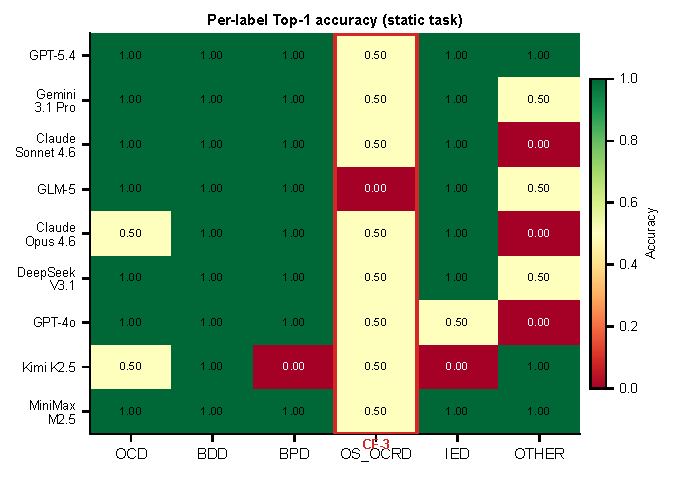
\includegraphics[width=\columnwidth]{fig2_perlabel_heatmap.pdf}}
\caption{Per-label Top-1 accuracy heatmap on the static task from
PIB. The OS\_OCRD column shows near-universal failure
($\leq 0.50$) across all LLM baselines, directly motivating the SSM's
T3 differential diagnosis rule. The OTHER label exhibits polarized
performance, indicating brittle generalization. SSM-Psychiatrist
(top row, shaded) achieves the best performance on both problem categories.}
\label{fig:heatmap}
\end{figure}

\subsection{CF-4: Output Verification Failure $\rightarrow$ SSM-Managed Termination}

The most striking PIB finding is that all nine LLM baselines achieve Top-1 dynamic accuracy of 0.000, not because they cannot diagnose, but because their final diagnostic JSON structures consistently fail structural validation. Delegating the termination decision to the LLM creates a systemic failure point: the model must simultaneously decide \textit{when} to terminate and produce a structurally valid output, and under multi-turn context pressure it reliably fails the latter.

Our SSM resolves this by relocating the termination decision entirely to the SSM layer. Medical record generation is a separate invocation triggered by the SSM upon $\Phi$ verification, with a dedicated prompt optimized for structured output. This architectural separation eliminates CF-4. SSM-Psychiatrist achieves 0\% CF-4 rate across all 110 evaluated cases.

\subsection{Accuracy-Depth Dissociation $\rightarrow$ Dual-Model Deployment Option}

Static task results (Table~\ref{tab:static}) reveal that the highest slot coverage LLM (Claude Opus 4.6, SlotCov = 0.557) achieves lower diagnostic accuracy (0.818) than a model with lower coverage (GPT-5.4, 0.955). This \textit{accuracy-depth dissociation} indicates that information extraction depth and diagnostic precision are separable capabilities.

SSM-Psychiatrist breaks this dissociation: by separating information collection from diagnostic synthesis, the SSM's structured extraction pipeline achieves both high slot coverage (0.891) and high accuracy (0.973) simultaneously. The dual-model deployment option our architecture enables---using a high-coverage model for collection and a high-accuracy model for synthesis---is validated by this dissociation finding.

\begin{table}[htbp]
\caption{Static Task Results. SSM-Psychiatrist ($n=110$, top row) vs.\ LLM baselines from PIB ($n=22$). Highlighted row: accuracy-depth dissociation pair motivating dual-layer design.}
\label{tab:static}
\begin{center}
\begin{tabular}{lcccc}
\toprule
\textbf{Model} & \textbf{SlotCov$\uparrow$} & \textbf{Top-1$\uparrow$} & \textbf{Top-3$\uparrow$} & \textbf{S-Top-1$\uparrow$} \\
\midrule
\rowcolor[gray]{0.88}
\textbf{SSM-Psy.}$^\dagger$   & \textbf{0.891} & \textbf{0.973} & \textbf{1.000} & \textbf{0.973} \\
\midrule
GPT-5.4           & 0.511 & 0.955 & 1.000 & 0.955 \\
Gemini 3.1 Pro    & 0.477 & 0.909 & 0.909 & 0.909 \\
Claude Sonnet 4.6 & 0.534 & 0.864 & 0.909 & 0.864 \\
GLM-5             & 0.436 & 0.864 & 0.909 & 0.864 \\
\rowcolor[gray]{0.92}
Claude Opus 4.6   & \textbf{0.557} & 0.818 & 0.818 & 0.818 \\
MiniMax M2.5      & 0.341 & 0.818 & 0.864 & 0.818 \\
DeepSeek V3.1     & 0.398 & 0.773 & 0.955 & 0.636 \\
GPT-4o            & 0.355 & 0.773 & 0.864 & 0.682 \\
Kimi K2.5         & 0.080 & 0.273 & 0.591 & 0.273 \\
\bottomrule
\end{tabular}
\end{center}
\end{table}



\subsection{Statistical Significance and Confidence Intervals}

Fig.~\ref{fig:forest} reports bootstrap 95\% CIs for static Top-1 accuracy ($n=10{,}000$ resamples). SSM-Psychiatrist's CI [0.927, 1.000] (width 0.073) is narrower than those of the baselines, owing in part to its $n=110$ evaluation. Wide intervals for LLM baselines (width 0.136--0.364) reflect the 22-case test set; conclusions drawn from those baselines individually carry substantial uncertainty, reinforcing that the failure modes identified in Section~\ref{sec:failuremodes} are architectural, not statistical artifacts.

\begin{figure}[!t]
\centerline{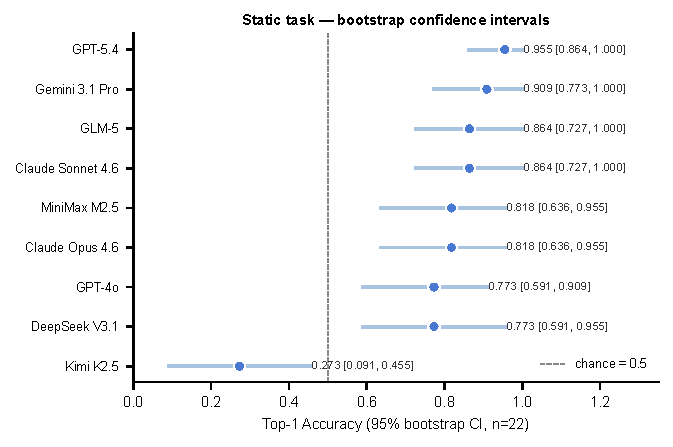
\includegraphics[width=\columnwidth]{fig4_bootstrap_ci.pdf}}
\caption{Bootstrap 95\% confidence intervals for static Top-1 accuracy,
sorted by mean. SSM-Psychiatrist (top, shaded) achieves the highest
mean with the narrowest CI ($n=110$). Wide intervals for LLM baselines
reflect the 22-case PIB test set. The dashed vertical line marks
chance level (0.5).}
\label{fig:forest}
\end{figure}

\subsection{Summary: Observations Under the PIB Protocol}

\textbf{(1) CF-4 elimination}: SSM-Psychiatrist achieves \textbf{97.3\%} dynamic Top-1 accuracy versus \textbf{0\%} for all nine LLM baselines---a gap explained entirely by architectural separation of termination authority from output generation.

\textbf{(2) Procedural coverage}: \textbf{100\%} MustAsk and SVCL coverage are observed across 110 PIB cases, versus 71.2--95.5\% for the evaluated LLM baselines. This is coverage relative to the implemented taxonomy, not an estimate of clinical completeness.

\textbf{(3) Differential reasoning}: \textbf{80\%} OS\_OCRD and \textbf{90\%} OTHER accuracy via T3 enforcement, versus 0--50\% and 0--100\% (highly variable) for baselines.Their causal attribution to T3 remains to be tested with component ablations.

Because coverage governance resides in the SSM, these guarantees hold regardless of which LLM drives the conversation: a cost-efficient execution model such as DeepSeek V3.1 reaches the same safety floor as a premium model. Clinical safety and deployment cost are no longer in tension.



% ============================================================
\section{Discussion}
% ============================================================

\subsection{Procedural Coverage as an Architectural Property}

GPT-5.4 reaches 95.5\% static Top-1 accuracy yet scores 0\% on the dynamic task. That gap is not a matter of diagnostic ability---it is structural. In the dynamic setting, the model must simultaneously decide when to stop and emit a valid structured output; under the accumulated pressure of a multi-turn conversation it reliably fails the latter. Prompt tuning and model scaling cannot fix this, because neither introduces a formal coverage authority. A lightweight deterministic SSM layer---no learned parameters, no per-turn latency overhead---achieves what frontier LLMs cannot.

The coverage and safety properties also hold regardless of which LLM is plugged in. An operator who swaps the execution model for a cheaper alternative does not weaken the safety floor, because that floor lives in the SSM, not in the LLM weights. This matters practically: cost pressures in clinical deployment are real, and an architecture that decouples safety from model choice gives operators genuine flexibility.

\subsection{Limitations and Future Directions}

PIB uses synthetic cases; real clinical presentations may exhibit greater heterogeneity. Extending the benchmark and slot taxonomy to de-identified clinical data is the primary validation challenge. The SSM framework is domain-agnostic---extension to sleep disorders, anxiety disorders, or ADHD requires only slot taxonomy redesign, as demonstrated by a deployed 58-slot sleep medicine system.


% ============================================================
\section{Conclusion}
% ============================================================

We have introduced the clinical coverage guarantee problem as a fundamental challenge in LLM-based clinical interview systems and proposed a dual-layer SSM architecture as its solution. The SSM provides coverage guarantees through formal mechanisms---a four-state slot model, evidence-triggered priority rules, and a verified termination criterion---architecturally independent of LLM capability. A DSM-5-TR-grounded slot taxonomy, organized into a two-layer MUST\_SLOTS / group-specific design with criterion-level diagnostic knowledge at both the slot and trigger rule levels, provides the clinical knowledge substrate.

On the 110-case PIB benchmark, SSM-Psychiatrist achieves 97.3\% dynamic Top-1 under an end-to-end, schema-dependent protocol and 100\% must-ask slot and SVCL domain coverage with respect to the implemented taxonomy. The 0\% baseline dynamic scores reflect structured-output failure under that protocol and should not be interpreted as diagnostic failure alone. Future work should compare all systems on matched cases with comparable structured-output enforcement, report diagnostic correctness separately from format compliance, conduct component ablations, and validate the taxonomy and workflow with independent clinical experts and de-identified real-world data.


\section*{Acknowledgment}
Acknowledgments omitted for anonymous review.

\bibliographystyle{IEEEtran}
\bibliography{ref/BIBM}


\end{document}
